\chapter{光电探测与光子计数：为什么数的是 n(n-1)}
\label{chap:e07}

\begin{chapteropening}
到上一章为止，我们已经把光"读"得很透了：光是一组模式的激发，每个模式就是一个谐振子，光子是模式里的一份能量，而数态、相干态、热态这三种光即使亮度相同，光子成对到达的倾向 \(b_2\) 却截然不同（第 \ref{chap:e06} 章）。可这一切都还停在"光态"这一侧。望远镜那一侧交回来的，从来不是一个波函数，而是一串冷冰冰的点击——某时刻，某像素，咔哒一声。本章要架的，正是这两侧之间的桥：光态究竟怎样变成探测器上的一串计数？我们会一步步弄清三件事。第一，为什么"探测一个光子"这件事，在数学上逼着我们去数 \(n(n-1)\) 而不是 \(n^2\)——那个被减掉的 \(n\)，正是"同一个光子不能和自己配对"。第二，怎样把一张事件表切成一格格时间门，用一个叫 Mandel \(Q\) 的数，一眼看出这束光比泊松更"抱团"还是更"规矩"。第三，为什么教科书上气势磅礴的 \(g^{(2)}(0)=2\)，到了真实望远镜上会缩水成 \(1+10^{-3}\) 甚至 \(1+10^{-6}\) 这样的小数——不是信号没了，而是被成千上万个模式稀释了。走完这一章，你手里就有了把"光的量子态"翻译成"可以真正拿去拟合的计数统计量"的全套换算。
\end{chapteropening}

\section{点击从哪来：探测就是吸收一个光子}
\label{sec:e07-absorption}

先回到最朴素的问题：探测器"看见"一个光子，物理上到底发生了什么？

不是光子撞上一面墙被弹回来，也不是它像小球一样被"接住"。真实的光电探测（photodetection）是一次\emph{吸收}：光场里一份能量被交给探测器（打出一个光电子、触发一次雪崩、翻转一个像素），与此同时，\textbf{光场里少了一个光子}。第 \ref{chap:e05} 章我们已经反复强调过这句话，并把它写成算符语言：吸收只用得上正频率场算符 \(\hat E^{(+)}\)，因为 \(\hat E^{(+)}\) 里装的是湮灭算符 \(\hat a\)（拿走一个光子），而不是产生算符 \(\hat a^\dagger\)。

现在只盯住一个模式。此时正频率场正比于该模式的湮灭算符，\(\hat E^{(+)}\propto\hat a\)。量子探测理论（Glauber）告诉我们一条干净的规则：\textbf{探测器在某一瞬间"咔哒"一声的概率，正比于把湮灭算符夹在光态里取平均。}一次点击对应一次吸收，所以单次点击率正比于

\begin{equation}
  p_1\ \propto\ \big\langle\,\hat E^{(-)}\hat E^{(+)}\,\big\rangle
  \ \propto\ \big\langle\,\hat a^\dagger\hat a\,\big\rangle
  =\langle\hat n\rangle .
  \label{eq:e07-single-click}
\end{equation}
\begin{formulaexplain}
单次点击概率正比于 \(\langle\hat a^\dagger\hat a\rangle=\langle\hat n\rangle\)。\(\hat a\) 先作用（吸收那一个光子），\(\hat a^\dagger\) 是它的厄米共轭；夹在一起取平均就是"平均有几个光子"。一句话：\emph{点击率跟着光子数走}。
\end{formulaexplain}

逐个符号交代。\(\hat E^{(+)}\)、\(\hat E^{(-)}=[\hat E^{(+)}]^\dagger\) 是正、负频率场算符（第 \ref{chap:e05} 章）；单模下它们分别正比于 \(\hat a\) 与 \(\hat a^\dagger\)，都无量纲（比例常数吸收进探测效率里）。\(\hat n=\hat a^\dagger\hat a\) 是光子数算符，本征值 \(N=0,1,2,\dots\)，纯整数无单位。尖括号 \(\langle\cdot\rangle\) 是对光态求量子期望。式 \eqref{eq:e07-single-click} 的物理含义再直白不过：想让探测器多响，就得让模式里平均光子多。这也是为什么在第 \ref{chap:e05} 章里，"每个模式其实很暗"（\(\bar n_\nu\sim10^{-2}\)）会直接翻译成"单个模式的点击率其实很低"。

\paragraph{两次符合点击：正规序自动扣掉"自己和自己配对"}
\label{sec:e07-normal-ordering}

真正有意思的是两次点击。设想我们问的不再是"响一声的概率"，而是"在（几乎）同一时刻响\emph{两}声的概率"——这正是 Hanbury Brown--Twiss 强度干涉、符合计数、二阶相干测量的核心量。两次点击意味着两次吸收：光场里\emph{接连}少了两个光子。按同样的探测规则，把两个 \(\hat E^{(+)}\) 排在一起，两次符合点击率正比于

\begin{equation}
  p_2\ \propto\ \big\langle\,\hat E^{(-)}\hat E^{(-)}\hat E^{(+)}\hat E^{(+)}\,\big\rangle
  \ \propto\ \big\langle\,\hat a^\dagger\hat a^\dagger\hat a\,\hat a\,\big\rangle .
  \label{eq:e07-two-click}
\end{equation}
\begin{formulaexplain}
两次符合点击概率正比于 \(\langle\hat a^\dagger\hat a^\dagger\hat a\hat a\rangle\)：所有湮灭算符（吸收）排在右边、所有产生算符排在左边。这种"产生在左、湮灭在右"的排法叫\textbf{正规序}（normal ordering），它正是"两次点击对应两次真实吸收"的数学写照。
\end{formulaexplain}

注意 \eqref{eq:e07-two-click} 里算符的次序：两个 \(\hat a\)（吸收）挨着排在最右，两个 \(\hat a^\dagger\) 排在最左。这个"湮灭全在右、产生全在左"的排列就叫正规序。它不是人为约定，而是探测的物理强加的：探测器只会对\emph{真实被吸收}的光子响应，所以每一次点击对应一个 \(\hat a\) 作用在态上，两次点击就把两个 \(\hat a\) 先后作用上去。

现在到了本章标题里那个问题的关键。式 \eqref{eq:e07-two-click} 里的算符组合 \(\hat a^\dagger\hat a^\dagger\hat a\hat a\) 到底等于什么？我们不猜，直接用第 \ref{chap:e05} 章反复用过的\emph{唯一}一条代数事实——对易关系 \([\hat a,\hat a^\dagger]=1\)，也就是 \(\hat a\hat a^\dagger=\hat a^\dagger\hat a+1\)——把它一步步化开。目标是把它写成数算符 \(\hat n=\hat a^\dagger\hat a\) 的函数。

先看数算符的平方：
\[
  \hat n^2=(\hat a^\dagger\hat a)(\hat a^\dagger\hat a)
  =\hat a^\dagger\,\underbrace{(\hat a\,\hat a^\dagger)}_{=\,\hat a^\dagger\hat a+1}\,\hat a
  =\hat a^\dagger(\hat a^\dagger\hat a+1)\hat a
  =\hat a^\dagger\hat a^\dagger\hat a\,\hat a+\hat a^\dagger\hat a .
\]
中间那一步就是把 \(\hat a\hat a^\dagger\) 换成 \(\hat a^\dagger\hat a+1\)，这是全推导用到的唯一非平凡代数。把右边第二项认出来是 \(\hat n\)，整理即得正规序与数算符的桥梁：
\begin{equation}
  \hat a^\dagger\hat a^\dagger\hat a\,\hat a
  =\hat n^2-\hat n
  =\hat n(\hat n-1).
  \label{eq:e07-normal-identity}
\end{equation}
\begin{formulaexplain}
正规序的双光子算符\emph{精确}等于 \(\hat n(\hat n-1)\)。若模式里有 \(N\) 个光子，可组的"有序光子对"是 \(N^2\)，但其中 \(N\) 个是"同一个光子与自己配对"；正规序自动把这 \(N\) 个假对减掉，剩下 \(N(N-1)\) 个\emph{真}对。
\end{formulaexplain}

这行式子值得停下来品味。它说的是：\textbf{正规序 = 自动扣掉自配对。}想象某个瞬间模式里恰有 \(N\) 个光子。若不动脑子，把"第一次数到的光子"和"第二次数到的光子"随意搭配，一共有 \(N\times N=N^2\) 种\emph{有序}选法。可其中有 \(N\) 种是"第一次和第二次数到的是\emph{同一个}光子"——这在物理上不可能，因为一次符合探测需要一个 START 脉冲和一个 STOP 脉冲，它们必须来自\emph{两次不同的吸收}，同一个光子被吸收后就没了，绝不会再触发第二声。于是真正可用的有序光子对数是 \(N(N-1)=N^2-N\)，那减掉的 \(N\) 正是自配对。式 \eqref{eq:e07-normal-identity} 里 \(\hat n^2\) 与 \(\hat n(\hat n-1)\) 差的那一项 \(\hat n\)，一个符号不多一个符号不少，就是这些自配对。

这也正是第 \ref{chap:e06} 章那个成对因子 \(b_2\) 的来历。回忆一下，我们在那里把单模零延迟成对倾向定义为
\[
  b_2\equiv\frac{\langle\hat n(\hat n-1)\rangle}{\langle\hat n\rangle^2},
\]
并算出数态给 \(b_2=1-1/n\)（反聚束）、相干态给 \(b_2=1\)（泊松基线）、热态给 \(b_2=2\)（聚束）。现在我们终于明白：分子上那个 \(\langle\hat n(\hat n-1)\rangle\) 不是谁拍脑袋定义的怪东西，而是探测器\emph{物理上只能数真对}的必然结果。把 \eqref{eq:e07-single-click} 与 \eqref{eq:e07-two-click} 归一化，就得到

\begin{equation}
  \frac{p_2}{p_1^2}\ \propto\
  \frac{\langle\hat a^\dagger\hat a^\dagger\hat a\hat a\rangle}{\langle\hat a^\dagger\hat a\rangle^2}
  =\frac{\langle\hat n(\hat n-1)\rangle}{\langle\hat n\rangle^2}
  =b_2 .
  \label{eq:e07-b2-from-clicks}
\end{equation}
\begin{formulaexplain}
把"两声一起响"的概率除以"两次独立响一声"的概率，就得到成对因子 \(b_2\)。它是探测器实测的量：\(b_2>1\) 光子爱抱团（聚束），\(b_2<1\) 光子相互回避（反聚束），\(b_2=1\) 各来各的（泊松）。
\end{formulaexplain}

一句话收束这一节：\textbf{探测器数的永远是"不同吸收事件"之间的关联，也就是 \(\langle n(n-1)\rangle\)，而不是一条连续波形，也不是 \(\langle n^2\rangle\)。}正规序不是形式主义的花招，它就是"一个光子只能被吸收一次"这条最硬的物理事实。图 \ref{fig:e07-factorial-moments} 把这件事画了出来：同一个计数分布，用 \(N^2\) 加权和用 \(N(N-1)\) 加权，权重差的就是那条自配对的对角线。

\begin{figure}[tbp]
\centering
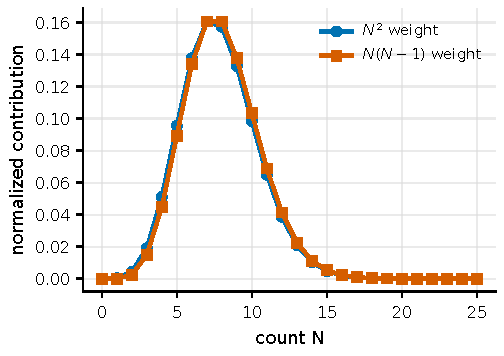
\includegraphics[width=0.86\linewidth]{figures/generated/chapter_04/ch04_factorial_moments.pdf}
\caption{普通二阶矩 \(N^2\) 与阶乘矩（factorial moment）\(N(N-1)\) 对不同光子数 \(N\) 的加权不同。符合探测只关心由\emph{不同}光子组成的有序对，因此正规序自动把 \(N^2-N(N-1)=N\) 这一项"同一光子与自己配对"的假贡献扣掉。这正是为什么二阶光子统计里出现的是 \(\langle N(N-1)\rangle\)，而不是 \(\langle N^2\rangle\)。}
\label{fig:e07-factorial-moments}
\end{figure}

\section{把事件表切成时间门：均值、方差与 Mandel 参数}
\label{sec:e07-time-gate}

上一节讲的是"瞬时"的算符期望。可真实望远镜交回来的是一张带时间戳的事件表——一长串"某个光子在某时刻到达"的记录（这张表的结构、时钟、死时间等硬件细节，留到第 \ref{chap:e13} 章细讲）。要把 \eqref{eq:e07-b2-from-clicks} 那样的算符期望，变成能真正从数据里算出来的数，我们需要一个具体的操作：\textbf{把连续时间切成一格一格宽度为 \(\Delta t\) 的"时间门"（time gate/bin），数每一格里落进了几个光子。}

设第 \(k\) 格时间门里的计数为 \(N_k\)（无量纲整数）。把许多格的计数收集起来，就得到一个计数分布 \(P(N)\)：出现 \(N\) 个光子的时间门占多大比例。对这个分布，我们关心两个最基本的统计量——均值和方差：

\begin{equation}
  \bar N=\langle N\rangle=\sum_{N=0}^{\infty}N\,P(N),
  \qquad
  \sigma_N^2=\big\langle N^2\big\rangle-\bar N^{\,2}
  =\sum_{N=0}^{\infty}(N-\bar N)^2\,P(N).
  \label{eq:e07-mean-var}
\end{equation}
\begin{formulaexplain}
\(\bar N\) 是每个时间门的\emph{平均}计数，\(\sigma_N^2\) 是计数在各门之间\emph{起伏}的大小（方差）。均值告诉你"平均多亮"，方差告诉你"忽明忽暗到什么程度"。判断光的量子性，看的是后者相对前者的大小。
\end{formulaexplain}

逐个交代：\(\bar N\) 无量纲，是门宽 \(\Delta t\) 内的平均光子数，等于计数率 \(r\)（单位 \(\mathrm{s^{-1}}\)）乘门宽，\(\bar N=r\,\Delta t\)。\(\sigma_N^2\) 也无量纲，是计数偏离均值的平方的平均。这里必须记住一件在天文里很反直觉的事：门宽 \(\Delta t\) 通常选得很小，比如 \(\Delta t=1\,\mathrm{ns}\)，而可见光点源的计数率也许只有 \(r=10^6\,\mathrm{s^{-1}}\)，于是

\[
  \bar N=r\,\Delta t=(10^6\,\mathrm{s^{-1}})(10^{-9}\,\mathrm{s})=10^{-3}.
\]

也就是说，\emph{一千个时间门里才有大约一个装着光子}，绝大多数门是空的（\(N=0\)），偶尔一个门里有 \(N=1\)，同一个门里有两个光子的机会小到 \(\sim10^{-6}\)。强度相关信号从来不是从一条肉眼可见的"光变曲线起伏"里读出来的，而是从 \(10^8\)、\(10^{12}\) 个时间门的微小统计偏差里，一点点累加出来的。这也是为什么我们必须用统计量、而不是用眼睛，来判断光的性质。

\paragraph{以泊松为零点：Mandel Q}
\label{sec:e07-mandel-q}

现在需要一把尺子，来量"这束光比随机到达更抱团、还是更规矩"。天然的零点是\textbf{泊松分布}（Poisson distribution）：若光子各来各的、彼此独立（相干态就是这样，见第 \ref{chap:e06} 章），计数服从泊松统计，它有一个招牌性质——\emph{方差恰好等于均值}：
\[
  \text{泊松：}\quad \sigma_N^2=\bar N .
\]
（这条我们在第 \ref{chap:e06} 章由 \(P(N)=e^{-\bar N}\bar N^N/N!\) 直接算过，是散粒噪声 shot noise 的定义。）把这条当零点，Mandel 用一个无量纲的数——\textbf{Mandel 参数}（Mandel \(Q\) parameter）——来度量偏离：

\begin{equation}
  Q\equiv\frac{\sigma_N^2-\bar N}{\bar N}.
  \label{eq:e07-mandel-q}
\end{equation}
\begin{formulaexplain}
\(Q\) 把泊松的 \(\sigma_N^2=\bar N\) 定为零点，量的是"方差比均值多出（或少掉）几成"。\(Q=0\) 泊松（相干态），\(Q>0\) 超泊松、光子抱团（热光），\(Q<0\) 亚泊松、光子过于规整（只能是非经典光）。
\end{formulaexplain}

逐项读。分子 \(\sigma_N^2-\bar N\) 是"方差超出泊松的部分"，分母 \(\bar N\) 把它无量纲化。三种情形，三种物理：

\begin{itemize}
  \item \textbf{\(Q=0\)（泊松，Poissonian）}：方差正好等于均值。光子独立随机到达，没有额外抱团也没有额外规整。理想稳定激光、相干态就在这里。
  \item \textbf{\(Q>0\)（超泊松，super-Poissonian）}：方差比均值大。光子倾向于\emph{成群}到来——某段时间强度偏高，多个光子挤着来；另一段偏低，一起变稀。这是热光、混沌光的招牌，也是 HBT 聚束的来源。
  \item \textbf{\(Q<0\)（亚泊松，sub-Poissonian）}：方差\emph{小于}均值，计数比随机情形更"规整"、更等间距。这没法用任何正的经典强度涨落解释，是货真价实的非经典信号（单光子源、共振荧光）。注意 \(Q\) 有下界：因为 \(N\ge0\)，可以证明 \(Q\ge-1\)，\(Q=-1\) 对应每个门里光子数完全固定的理想数态。
\end{itemize}

举个数量级。单模热光在门宽 \(\Delta t\) 内的计数服从玻色--爱因斯坦分布，方差为 \(\sigma_N^2=\bar N+\bar N^2\)（第 \ref{chap:e06} 章）。代入 \eqref{eq:e07-mandel-q}：
\[
  Q_{\rm th}=\frac{(\bar N+\bar N^2)-\bar N}{\bar N}=\bar N .
\]
理想单模热光的 \(Q\) 就等于它自己的平均计数——听上去可观，但别忘了，可见光每模式弱光极限下 \(\bar n_\nu\sim10^{-2}\)（第 \ref{chap:e05} 章），所以哪怕是纯净单模热光，\(Q\) 本身也只有百分之几。真实多模观测会把它压得更低，这正是下一节的主题。

\section{从 Mandel Q 到 g(2)(0)：一条代数恒等式}
\label{sec:e07-q-to-g2}

我们现在有了两套语言：一套是"光子成对到达"的语言，主角是 \(g^{(2)}(0)=\langle N(N-1)\rangle/\bar N^2\)（它就是上一章 \(b_2\) 的时间门版本，也是第 \ref{chap:e08} 章二阶相干函数在零延迟的取值）；另一套是"计数方差"的语言，主角是 Mandel \(Q\)。这两套说的其实是同一件事，把它们\emph{精确}连起来的，只是一条初中代数恒等式。

关键的一步是把阶乘矩 \(\langle N(N-1)\rangle\) 用均值和方差表示。展开 \(N(N-1)=N^2-N\)，两边取平均：
\[
  \big\langle N(N-1)\big\rangle=\big\langle N^2\big\rangle-\langle N\rangle
  =\big\langle N^2\big\rangle-\bar N .
\]
再用方差的定义 \(\sigma_N^2=\langle N^2\rangle-\bar N^2\)，即 \(\langle N^2\rangle=\sigma_N^2+\bar N^2\)，代进去：
\begin{equation}
  \big\langle N(N-1)\big\rangle=\sigma_N^2+\bar N^{\,2}-\bar N .
  \label{eq:e07-identity}
\end{equation}
\begin{formulaexplain}
一条纯代数恒等式：阶乘矩 = 方差 + 均值平方 \(-\) 均值。它把"成对语言"里的 \(\langle N(N-1)\rangle\) 换算成"方差语言"里的 \(\sigma_N^2\) 和 \(\bar N\)，是连接 \(g^{(2)}(0)\) 与 \(Q\) 的唯一桥梁。
\end{formulaexplain}

这里没有任何物理近似，纯粹是把 \(N(N-1)\) 拆开重排，对\emph{任何}计数分布都成立。现在把它代进 \(g^{(2)}(0)\) 的定义。除以 \(\bar N^2\)：
\[
  g^{(2)}(0)=\frac{\langle N(N-1)\rangle}{\bar N^{\,2}}
  =\frac{\sigma_N^2+\bar N^{\,2}-\bar N}{\bar N^{\,2}}
  =\underbrace{\frac{\bar N^{\,2}}{\bar N^{\,2}}}_{=1}
  +\frac{\sigma_N^2-\bar N}{\bar N^{\,2}} .
\]
把最后一项的分子分母同时看一眼：\(\sigma_N^2-\bar N\) 正是 Mandel \(Q\) 的分子，而 \(Q=(\sigma_N^2-\bar N)/\bar N\)，所以 \((\sigma_N^2-\bar N)/\bar N^2=Q/\bar N\)。于是

\begin{equation}
  g^{(2)}(0)=\frac{\langle N(N-1)\rangle}{\bar N^{\,2}}
  =1+\frac{Q}{\bar N}.
  \label{eq:e07-g2-q}
\end{equation}
\begin{formulaexplain}
零延迟二阶相干 \(g^{(2)}(0)\) 与 Mandel \(Q\) 只差一个 \(\bar N\)。\(Q\) 度量绝对的方差过剩，\(g^{(2)}(0)\) 度量归一化后的成对过剩；平均计数 \(\bar N\) 越小，同样的 \(Q\) 会撬起越大的 \(g^{(2)}(0)-1\)。
\end{formulaexplain}

逐项交代：\(g^{(2)}(0)\) 无量纲，\(=1\) 是独立到达基线，\(>1\) 聚束，\(<1\) 反聚束。\(Q\) 无量纲，\(\bar N\) 无量纲。式 \eqref{eq:e07-g2-q} 是本章最实用的一条换算：它把"方差语言"和"成对语言"锁在一起。用它验一下自洽——单模热光 \(Q_{\rm th}=\bar N\)，代入得 \(g^{(2)}(0)=1+\bar N/\bar N=2\)，正是第 \ref{chap:e06} 章的热光聚束峰；相干态 \(Q=0\)，得 \(g^{(2)}(0)=1\)，泊松基线。两头都对上了。

式 \eqref{eq:e07-g2-q} 还藏着一个天文观测的关键教训，图 \ref{fig:e07-mandel-q-g2} 把它画了出来：\(\bar N\) 在分母上。当平均计数很低（弱光极限）时，一个很小的 \(Q\) 也能对应一个明显偏离 1 的 \(g^{(2)}(0)\)；反过来，把时间门加宽会让 \(\bar N\) 变大、也会把许多互不相干的时间模式平均进同一个 \(N\)，两头一起把 \(g^{(2)}(0)-1\) 稀释掉。所以有一条铁律，务必写进任何一份强度相关的报告里：

\begin{quote}
\textbf{只报 \(g^{(2)}(0)\) 或只报 \(Q\) 都是不完整的。}必须同时给出四样东西：\(Q\)（或 \(g^{(2)}(0)-1\)）、\textbf{时间门宽 \(\Delta t\)}、\textbf{有效模式数 \(M\)}、\textbf{平均计数 \(\bar N\)}。缺一个，别人就无法判断你测到的是内禀信号还是被门宽稀释后的残影。
\end{quote}

\begin{figure}[tbp]
\centering
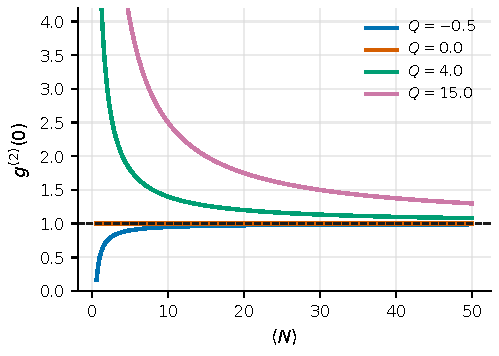
\includegraphics[width=0.86\linewidth]{figures/generated/chapter_04/ch04_mandel_q_g2.pdf}
\caption{在固定时间门内，Mandel \(Q\) 通过 \(g^{(2)}(0)=1+Q/\bar N\) 决定零延迟二阶相干。平均计数 \(\bar N\) 越低，同样的 \(Q\) 撬起的 \(g^{(2)}(0)-1\) 越大；把时间门加宽或平均更多模式，\(\bar N\) 增大、\(Q\) 被稀释，曲线逐渐回落到泊松基线 1。这解释了为什么报告二阶相关时必须同时注明门宽、模式数与平均计数。}
\label{fig:e07-mandel-q-g2}
\end{figure}

\section{多模稀释：为什么天文里的 excess 是小数而不是 1}
\label{sec:e07-multimode}

教科书上，单模热光的聚束峰堂堂正正是 \(g^{(2)}(0)=2\)，也就是 excess \(g^{(2)}(0)-1=1\)。可翻开任何一篇真实的天文强度干涉论文，你看到的峰高却是 \(10^{-3}\)、\(10^{-6}\) 这样卑微的小数。信号是不是丢了?没有。它是被\emph{多模平均}稀释了。这一节把稀释算清楚。

回忆第 \ref{chap:e05} 章：天文里"一个通道"几乎从来不是单单一个量子模式，而是 \(M\) 个独立模式的总和，\(M\simeq(\Delta t/\tau_c)(A\Omega/\lambda^2)N_{\rm pol}\)，可见光下轻易上千上万。现在把这句话的统计后果算出来。

设探测到的总计数 \(N\) 是 \(M\) 个\emph{独立、强度相近}的热光模式贡献之和，每个模式的平均计数为 \(m=\bar N/M\)。对单个热模，方差是 \(m+m^2\)（玻色--爱因斯坦，第 \ref{chap:e06} 章）。独立随机变量相加，\textbf{均值相加、方差也相加}（这是概率论里独立变量方差可加这一标准结论，我们直接引用）。于是总方差为
\[
  \sigma_N^2=\sum_{i=1}^{M}(m+m^2)=M m+M m^2
  =\underbrace{Mm}_{=\bar N}+M\Big(\frac{\bar N}{M}\Big)^2 .
\]
第一项 \(Mm=\bar N\) 就是总均值（散粒噪声那一份），第二项化简 \(M\cdot\bar N^2/M^2=\bar N^2/M\)。于是

\begin{equation}
  \sigma_N^2=\bar N+\frac{\bar N^{\,2}}{M}.
  \label{eq:e07-multimode-var}
\end{equation}
\begin{formulaexplain}
\(M\) 个独立热模平均后，方差的两部分：\(\bar N\) 是绕不开的散粒噪声，\(\bar N^2/M\) 是热光的额外"波动噪声"。模式越多（\(M\) 越大），第二项被摊得越薄，光就越像泊松。
\end{formulaexplain}

逐项交代：\(\bar N\) 是总平均计数（无量纲），\(M\) 是有效模式数（无量纲，\(\ge1\)），\(\bar N^2/M\) 是被 \(M\) 稀释后残留的超泊松涨落。现在把 \eqref{eq:e07-multimode-var} 塞进 Mandel \(Q\) 和 \(g^{(2)}(0)\)。先算 \(Q\)：
\[
  Q=\frac{\sigma_N^2-\bar N}{\bar N}
  =\frac{\bar N^2/M}{\bar N}=\frac{\bar N}{M}.
\]
再用换算式 \eqref{eq:e07-g2-q}：
\begin{equation}
  g^{(2)}(0)=1+\frac{Q}{\bar N}=1+\frac{1}{M}.
  \label{eq:e07-multimode-g2}
\end{equation}
\begin{formulaexplain}
\(M\) 个独立热模平均后，聚束峰高从单模的 \(g^{(2)}(0)-1=1\) 掉到 \(1/M\)。这一条 \(1/M\) 定律，就是天文强度干涉里 excess 总是小数的根源。
\end{formulaexplain}

这条 \(g^{(2)}(0)=1+1/M\) 干净得惊人，物理也清楚：\(M\) 个独立模式的强度涨落各自随机、互相抵消，平均下来强度越来越平稳，聚束这种"抱团"效应就被摊薄了 \(M\) 倍。\(M=1\) 给经典的 2；\(M=1000\) 给 \(1+10^{-3}\)；\(M=10^6\) 给 \(1+10^{-6}\)。这就是为什么天文 HBT 图上直接读到的从来不是雄伟的 2，而是要从海量事件对里刨出来的小数 excess。

那些 \(M\) 从哪来？逐个数（都在第 \ref{chap:e05} 章的模式计数框架里）：

\begin{itemize}
  \item \textbf{偏振（2 模）}：若不把偏振投影到单一通道，两个正交偏振各自是独立的热模，\(M_{\rm pol}\simeq2\)，一下就把理想峰从 2 压到 1.5。
  \item \textbf{空间散斑（speckle）}：被大气抖动（seeing）糊开的像、或耦合进粗光纤、或落在大像素上，会同时收进许多空间模式，\(M_{\rm sp}=A\Omega/\lambda^2\) 可以很大。
  \item \textbf{宽谱多频模}：滤光片越宽，带宽 \(\Delta\nu\) 内独立频率模式越多。
  \item \textbf{门宽 \(>\) 相干时间}：这是最狠的一项。可见光相干时间 \(\tau_c\sim1\,\mathrm{ps}\)，而最快探测器时间响应 \(\sim100\,\mathrm{ps}\)–\(1\,\mathrm{ns}\)，一个时间门里就压进了 \(\Delta t/\tau_c\sim10^2\)–\(10^3\) 个独立时间模式，单这一项就把 excess 压低两三个数量级。
\end{itemize}

代入一组真实标尺（取自恒星热光聚束实验）：中心波长约 \(7800\,\text{\AA}\)、最窄滤光片 \(10\,\text{\AA}\)，对应 \(\Delta\nu\simeq5\times10^{11}\,\mathrm{Hz}\)、相干时间 \(\tau_c\simeq1.6\)–\(2\,\mathrm{ps}\)；APD 单光子时间抖动约 \(500\,\mathrm{ps}\)，两只探测器的相对响应峰宽约 \(700\,\mathrm{ps}\)。光是"门宽/相干时间"这一项就贡献 \(M\sim700\,\mathrm{ps}/2\,\mathrm{ps}\sim350\) 倍稀释，再叠上偏振和空间模式，理想的 \(g^{(2)}(0)=2\) 就被压到观测峰 \(g^{(2)}(0)-1\sim10^{-3}\) 这个量级——实验里对三颗亮星测到的正是 \(10^{-3}\) 量级的聚束峰 \citep{2017MNRAS.472.4126G}。所以再强调一次：望远镜相关图上出现的 \(1+10^{-3}\)、\(1+10^{-6}\)，不是"没有聚束"，而是"聚束被 \(M\) 稀释"。要把 \(M\) 从数据里除干净，才能还原源本身的物理。这套稀释账，会在第 \ref{chap:e08} 章的 Siegert 关系和第 \ref{chap:e10} 章的空间强度干涉里反复用到。

\section{探测器不是理想的：效率、背景与死时间}
\label{sec:e07-nonideal}

到此为止我们假装探测器是完美的：每个到达的光子都被数到，没有噪声，数完立刻能数下一个。真实探测器三样都不满足。这一节把三种非理想性各讲一句物理，好在其中两种恰好能沿用我们已经建立的语言，第三种留个引子给第 \ref{chap:e13} 章。图 \ref{fig:e07-detection-loss} 把效率损耗与背景稀释这两条主线画在一起。

\paragraph{效率 η：损耗就像一块分束镜}
\label{sec:e07-efficiency}

真实探测器的量子效率（quantum efficiency）\(\eta<1\)：平均每 \(1/\eta\) 个到达的光子才被数到一个。怎样给这件事建模？有一个漂亮又准确的图像：\textbf{损耗完全等价于在光路上插一块透射率为 \(\eta\) 的分束镜（beamsplitter）}，透射的那一份 \(\eta\) 被数到，反射掉的 \(1-\eta\) 丢失，而分束镜的另一个入口漏进真空涨落。

这个图像的力量在于，它把"损耗"变成了"每个光子独立地以概率 \(\eta\) 存活"——这在概率论里叫\textbf{二项稀释}（binomial thinning）。而稀释一个分布有一条关键性质：它对\emph{泊松}分布是封闭的（泊松稀释后还是泊松），对超泊松分布则\emph{朝泊松方向拉}。

我们把这件事算到底，看看 Mandel \(Q\) 究竟怎么变。设某个时间门里\emph{到达}的光子数是随机变量 \(N\)（均值 \(\bar N\)、方差 \(\sigma_N^2\)），\emph{被数到}的计数是 \(M\)。二项稀释的意思是：给定 \(N\)，每个光子各自以概率 \(\eta\) 独立存活，于是条件分布是二项分布 \(M\mid N\sim\mathrm{Binomial}(N,\eta)\)，其条件均值与条件方差是二项分布的标准结果
\[
  \mathbb E[M\mid N]=\eta N,\qquad
  \operatorname{Var}(M\mid N)=N\,\eta(1-\eta).
\]
均值直接取期望：\(\bar M=\mathbb E[\eta N]=\eta\bar N\)。方差则要用\textbf{全方差公式}（law of total variance）\(\operatorname{Var}(M)=\mathbb E[\operatorname{Var}(M\mid N)]+\operatorname{Var}(\mathbb E[M\mid N])\)——它把总起伏拆成"每个 \(N\) 内部的二项抖动"和"\(N\) 本身在各门之间的起伏"两部分，是处理"随机个数里再随机存活"这类两层随机的标准工具。逐项代入：
\[
  \sigma_M^2
  =\underbrace{\mathbb E\big[N\,\eta(1-\eta)\big]}_{=\,\eta(1-\eta)\bar N}
  +\underbrace{\operatorname{Var}(\eta N)}_{=\,\eta^2\sigma_N^2}
  =\eta(1-\eta)\bar N+\eta^2\sigma_N^2 .
\]
第一项是损耗自己引入的二项散粒噪声，第二项是原起伏被 \(\eta^2\) 缩小后的残留。把 \(\bar M=\eta\bar N\) 和这个 \(\sigma_M^2\) 一起塞进 Mandel 参数的定义 \eqref{eq:e07-mandel-q}：
\[
  Q_M=\frac{\sigma_M^2-\bar M}{\bar M}
  =\frac{\eta(1-\eta)\bar N+\eta^2\sigma_N^2-\eta\bar N}{\eta\bar N}
  =\frac{\eta^2\sigma_N^2-\eta^2\bar N}{\eta\bar N}
  =\eta\,\frac{\sigma_N^2-\bar N}{\bar N}=\eta\,Q .
\]
中间那一步用到 \(\eta(1-\eta)\bar N-\eta\bar N=-\eta^2\bar N\)，把两项散粒噪声合并，剩下的正好整体提出一个 \(\eta\)。于是稀释把均值和方差过剩都按比例缩小，\(\bar N\to\eta\bar N\)，而
\[
  Q\ \longrightarrow\ \eta\,Q .
\]
一句话物理：

\begin{quote}
\textbf{损耗随机地删掉光子，把超泊松统计朝泊松零点拽。}\(\eta\to0\) 时任何光的计数都退化成泊松——这也是为什么效率极低的探测会"抹平"量子特征。
\end{quote}

但这里有一个救命的细节，务必记牢：\emph{归一化后的} \(g^{(2)}(0)\) 对损耗\textbf{免疫}。因为 \(Q\to\eta Q\) 而 \(\bar N\to\eta\bar N\)，代进 \eqref{eq:e07-g2-q}：
\[
  g^{(2)}(0)=1+\frac{\eta Q}{\eta\bar N}=1+\frac{Q}{\bar N}\quad(\text{不变}).
\]
分子分母上的 \(\eta\) 精确约掉。物理上这很合理：损耗只是随机地少数了一些光子，并不会改变"剩下的光子成对到达的\emph{倾向}"。这正是强度干涉即使在效率不高、光子稀少的天文条件下仍然可行的根本原因——\(g^{(2)}(0)-1\) 这个我们真正要测的量，不怕损耗。损耗伤的是\emph{信噪比}（少了光子就少了事件对，统计误差变大），而不是信号的\emph{数值}。

\paragraph{背景稀释：源光子只占一部分}
\label{sec:e07-background}

第二种非理想性是背景光：天光、月光、暗计数、邻近天体，都会在同一个通道里贡献与源无关的计数。设源光子只占总计数的比例为 \(f\)（source fraction，\(0<f\le1\)），其余 \(1-f\) 是不相关的背景。背景自己不带聚束峰（它是独立泊松的），而一次两光子符合要求\emph{两}个光子都来自源——每个各带一个因子 \(f\)。于是测到的 excess 被 \(f^2\) 压低：
\begin{equation}
  g^{(2)}_{\rm obs}(0)-1\simeq f^2\big[g^{(2)}_{\rm src}(0)-1\big].
  \label{eq:e07-background}
\end{equation}
\begin{formulaexplain}
背景把源信号按 \(f^2\) 稀释：两次点击都得是源光子才算数，各出一个 \(f\)。源只占一半（\(f=0.5\)）时，聚束峰就掉到原来的四分之一。
\end{formulaexplain}

逐项交代：\(f\) 是源计数占总计数的比例（无量纲），\(g^{(2)}_{\rm src}(0)\) 是源本身的二阶相干，\(g^{(2)}_{\rm obs}(0)\) 是掺了背景后测到的。这条 \(f^2\) 律和多模稀释的 \(1/M\) 是并列的两道关卡：一个来自"通道里混了多少无关模式"，一个来自"计数里混了多少无关背景"。做误差预算（第 \ref{chap:e15} 章会系统展开）时，两者都要老老实实乘进去。

\paragraph{死时间与后脉冲：留给第 13 章}
\label{sec:e07-deadtime}

第三种非理想性是探测器数完一个光子后，有一小段\emph{死时间}（dead time）不能再响应（单光子探测器常有 \(10\)–\(100\,\mathrm{ns}\)），以及触发后偶尔冒出的假计数（后脉冲，afterpulsing）。这两样会在\emph{零延迟附近}的自相关里挖坑、造假峰，恰好污染我们最想看的地方。它们不改变本章"数 \(n(n-1)\)"的基本规则，但会扭曲实测的相关峰形，需要专门的硬件对策（最常见的是用分束镜把光分到两只独立探测器做交叉相关，绕开单探测器的死时间）。这些属于探测器与事件表的硬件细节，我们留到第 \ref{chap:e13} 章专门处理，此处只提一句、按下不表。

\begin{figure}[tbp]
\centering
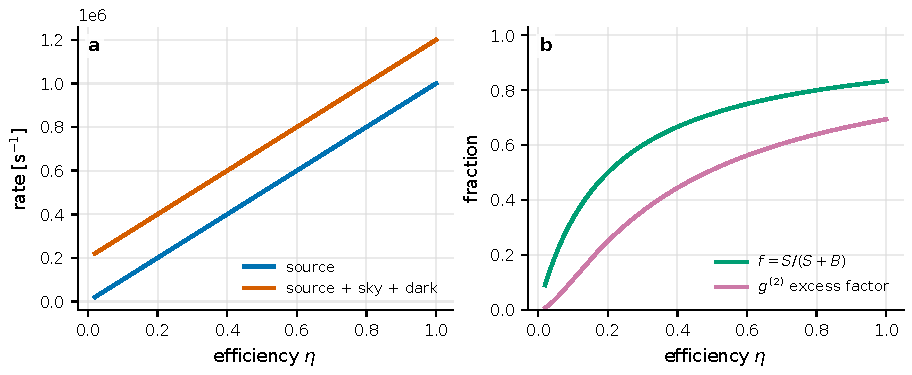
\includegraphics[width=0.85\linewidth]{figures/generated/chapter_03/ch03_detection_loss_background.pdf}
\caption{两种把观测统计朝泊松基线拉的非理想效应。效率损耗 \(\eta\) 等价于一块分束镜的二项稀释，随机删掉光子、把 Mandel \(Q\) 按 \(Q\to\eta Q\) 压向零点（但归一化后的 \(g^{(2)}(0)\) 不变）；背景稀释则把源信号按源光子占比 \(f\) 的平方 \(f^2\) 压低。二者与多模稀释 \(1/M\) 一起，构成天文强度相关信号被压成小数 excess 的三道关卡。}
\label{fig:e07-detection-loss}
\end{figure}

\section{本章要点}
\label{sec:e07-summary}

\begin{itemize}
  \item \textbf{探测就是吸收，所以数的是正规序。}单次点击率 \(\propto\langle\hat a^\dagger\hat a\rangle=\langle\hat n\rangle\)；两次符合点击率 \(\propto\langle\hat a^\dagger\hat a^\dagger\hat a\hat a\rangle=\langle\hat n(\hat n-1)\rangle\)。用 \([\hat a,\hat a^\dagger]=1\) 可精确证明 \(\hat a^\dagger\hat a^\dagger\hat a\hat a=\hat n(\hat n-1)\)。
  \item \textbf{\(n(n-1)\) 而非 \(n^2\)，是因为自配对被扣掉。}一个 START 和一个 STOP 必来自两次\emph{不同}吸收；\(N^2\) 里那 \(N\) 个"同一光子配自己"的假对被正规序自动减去，剩 \(N(N-1)\) 个真对，正是第 \ref{chap:e06} 章 \(b_2\) 分子的来历。
  \item \textbf{时间门 + Mandel \(Q\)。}把事件表切成宽 \(\Delta t\) 的门，数 \(N\)，得 \(\bar N=r\Delta t\)、\(\sigma_N^2\)；\(Q=(\sigma_N^2-\bar N)/\bar N\) 以泊松为零点：\(Q=0\) 泊松，\(Q>0\) 超泊松（热光），\(Q<0\) 亚泊松（非经典）。
  \item \textbf{一条恒等式连起两套语言。}由 \(\langle N(N-1)\rangle=\sigma_N^2+\bar N^2-\bar N\) 推得 \(g^{(2)}(0)=1+Q/\bar N\)。报告时必须同时给出 \(Q\)、门宽 \(\Delta t\)、模式数 \(M\)、平均计数 \(\bar N\)，缺一不可。
  \item \textbf{多模稀释的 \(1/M\) 律。}\(M\) 个独立热模平均后 \(\sigma_N^2=\bar N+\bar N^2/M\)，\(g^{(2)}(0)=1+1/M\)。偏振（2）、空间散斑、宽谱多频模、门宽 \(>\tau_c\) 都贡献 \(M\)，这就是天文 excess 常是 \(10^{-3}\)、\(10^{-6}\) 而非 1 的原因。
  \item \textbf{探测非理想。}效率 \(\eta\) 像分束镜，二项稀释把 \(Q\to\eta Q\)（超泊松被拉向泊松），但归一化的 \(g^{(2)}(0)\) 不变；背景把信号按 \(f^2\) 压低；死时间/后脉冲留待第 \ref{chap:e13} 章。
\end{itemize}

\medskip
\noindent\textbf{想一想。}
\begin{enumerate}
  \item 一束单模热光测得 \(g^{(2)}(0)=2\)。若把时间门宽从 \(1\,\mathrm{ps}\) 加宽到 \(1\,\mathrm{ns}\)（相干时间仍是 \(1\,\mathrm{ps}\)），有效时间模式数变成多少？此时 \(g^{(2)}(0)-1\) 大约掉到多少？
  \item 探测效率 \(\eta\) 从 \(0.5\) 掉到 \(0.05\)，测到的 \(g^{(2)}(0)-1\) 会变吗？Mandel \(Q\) 会变吗？分别说明为什么。
  \item 观测中源光子只占总计数的 \(f=1/3\)，其余是天光背景。若源本身是单模热光（\(g^{(2)}_{\rm src}(0)=2\)），你在这个通道里测到的 \(g^{(2)}_{\rm obs}(0)\) 大约是多少？
\end{enumerate}
